%\documentclass{article}
%\usepackage{graphicx}
\documentclass[10pt,conference]{IEEEtran}

%%% include required packages

\usepackage{amsmath,amssymb,amsfonts}   % ams packages, useful for typing math
\usepackage{bm}                         % bm provides \boldmath for bold fonts in equations (matrices, vectors)
\usepackage{graphicx}                   % needed to insert EPS graphics via \includegraphics
\usepackage{psfrag}                     % needed only if text in EPS graphics shall be replaced (e.g., formulas in graphics)

\usepackage{hyperref}

%%% define macros
\newcommand{\compl}{\mathbb{C}}         % complex number field, e.g., x \in \compl 
\newcommand{\real}{\mathbb{R}}          % real number field, e.g., x \in \real
% if you have too many, put them in a separate file, e.g., macros.tex
% and include here via \input{macros}


%%%%%%%%%%%%%%%%%%%%%%%%%%%%%%%%%%%%%%%%%%%%%%%%%%%
%%% Main body of the document
%%%%%%%%%%%%%%%%%%%%%%%%%%%%%%%%%%%%%%%%%%%%%%%%%%%

\begin{document}

\title{Random Beamforming Methods for Compressive Sensing Based Direction of Arrival Estimation}
\author{\textbf{Sunita Silwal, Sergii Skolikov}\\
Electronic Measurement Technik\\
Ilmenau University of Technology\\                      
98693 Ilmenau, Germany\\
Email: sunita.silwal@tu-ilmenau.de}
\maketitle
\begin{abstract}
Compressive Sensing  a novel research area, has attracted a lot of attention in many real world systems such as imaging, analog to digital converter, radar, sonar, wireless communication  and electrical engineering in recent years. Compressive Sensing makes it feasible to recover the signals from the small set of measurements below the rate defined by Nyquist Sampling theorem. While estimating the Direction of Arrival (DoA), CS is a good approach which helps to reduce the complexity caused by a larger number of antenna array element. It helps to reduce the bigger matrix size while perfectly reconstructing the information from the sparse signal.However, the main goal in CS is to develop the measurement matrix such that the measurement matrix(sensing matrix) doesn't destroy the original signal.  In this paper, we will focus on how to develop the structured random sensing matrix which will help to obtain the perfect information of high dimensional sparse signal exactly even after the reduction in the dimension. 


	
\end{abstract}


\textbf{Keywords:} \textit{DoA estimation, Compressive Sensing. Random sequence, Sensing matrix}
\section{Introduction}
Direction of arrival(DoA) estimation of the propagating plane or \textit{direction finding} has been an active area of research in various different field such as wireless communication, radar, sonar, navigation, radio astronomy etc. In Wireless communication, it is mainly focused on estimating the direction of electromagnetic waves striking on one or more antenna elements \cite{tuncer2009classical}. In this paper we deal with the DoA estimation with the conventional concept of Compressive Sensing. 

 In the figure \ref{Ula}, we can see $M$-antenna element Uniform Linear array which helps to provide a better performance than a single antenna element. Different research in DOA tells us, higher the number of antenna elements in an array the better is the angular resolution of the estimated DoA but, it results in increase in complexity in both hardware and software (DEUCSAP). Increase in number of frontend circuit leads the software to deal with the larger size data matrices. Compressive Sensing (CS) addresses this insufficiencies which is a method for capturing the information stored in the sparse signal and reconstructing it back from the compressed measurements.
\begin{figure} [!htb]
\centering
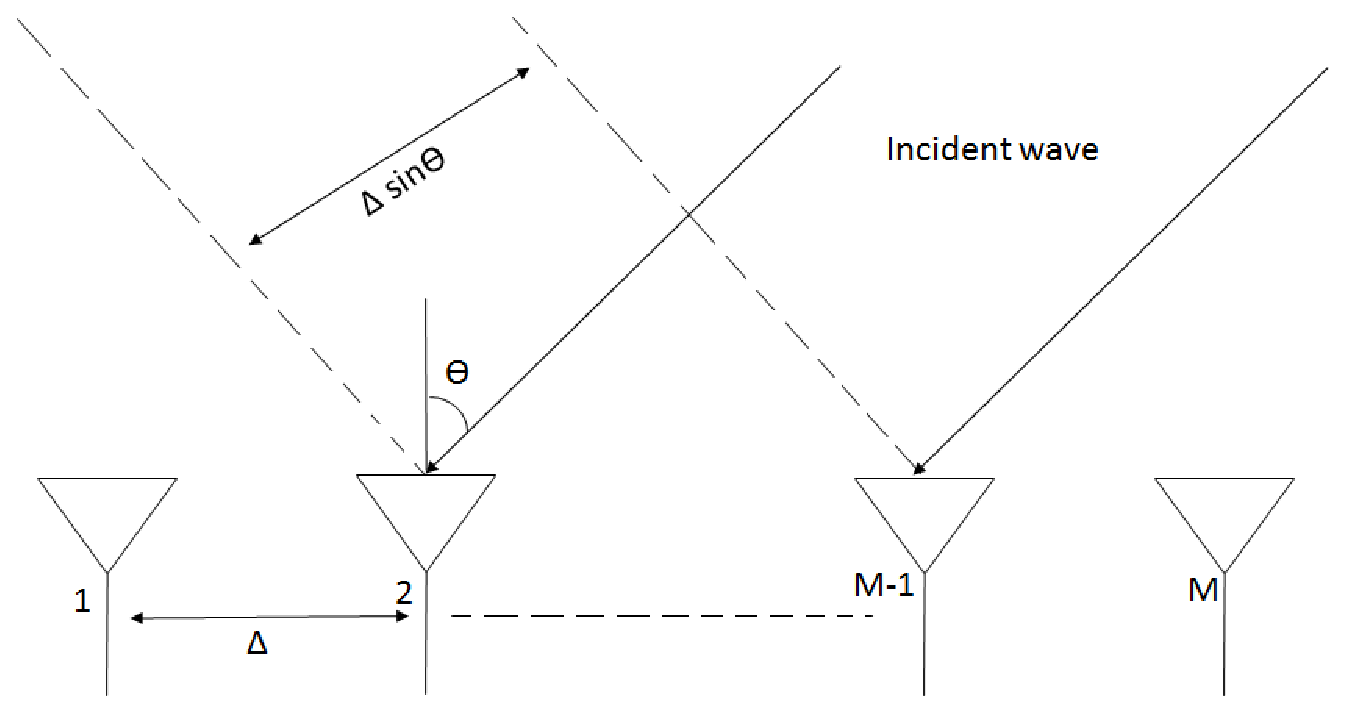
\includegraphics[scale=.35]{Ula.eps}
\caption{Plane wave on ULA antenna }
\label{Ula}
\end{figure}

Since the past few years, compressive sensing has been rising as a revolutionary sampling paradigm in signal processing. Nyquist Shannon sampling theorem used in Signal processsing states that in order to perfectly reconstruct any bandlimited signal, a certain minimum number of samples is required. However, by using the compressive sampling (CS) algorithm, we can reconstruct the original signal $ x \in \mathbb{R}^{M} $ showed that a signal having a sparse representation can be recovered exactly from a small set of linear , nonadaptive measurements ($'m'$ measurement where $m < M$). The signal \textit{x} is said to be $K$-sparse if it can be perfectly reconstructed back by using $K<<M$ coefficients where, $x(t)=As$ and $A$ is the array manifold matrix formed by the array steering vectors of the Uniform Linear Array (ULA). 


According to the Compressive Sensing theory, the signal x can be perfectly reconstructed from the general linear measurement with $y(t)= \Phi x(t)$ (). Here, $\Phi$ is the measurement matrix which is constructed from the context of the system. This matrix should satisfy the Restricted Isometric Property (RIP).

The Sensing matrix $\Phi$ should be fixed that is it should not depend on the signal $x$ and should be incoherent with the Array Steering matrix. As defined in (), while designing the sensing matrix $\Phi$ two conditions must be satisfied, first, the dimensionality reduction from $m$ to $M$ measurements  should not damage the salient information  of the sparse signal and second, there should be proper reconstruction algorithm. The design procedure of measurement or the sensing matrix plays a significant role in compressive sensing as it provides the original signal without information loss and any other prior knowledge. 

The incoherence of $\Phi$ is ensured by the randomness in the matrix component. The measurement matrix or the sensing matrix is constructed from the random sequence. In this paper, we will discuss about three different frameworks to build the random sequence and thus the overall sensing matrix for $\Phi$.

The remaining of the paper is organised as follows: In section \ref{a} we will first discuss about the system model. In section \ref{b}, we will discuss on different random sequence generation methods for the sensing matrix for Compression Sensing. Based on these methods , we will simulate and see the results on section \ref{d} and conclusion in section \ref{e}.
\section{System Model}  \label{a}
Here, we consider $K$ narrowband planar wavefront from $K$- sources impinging in the far field of an $M$-element antenna array at $\theta_{k}$ azimuth angle. Then, the received signal at the antenna array of $M$-sensors can be written as (),
\begin{equation} \label{1}
x(t)= \sum_{k=1}^{K}a(\theta_{k})*s_{k}(t)+w(t)
\end{equation} 

where $s_{k}(t)$,$ k = 1, 2, . . . , K$, is a  narrowband planar wavefront transmitted from $k$-th source, $w(t)$ is an $M × 1$ vector representing the additive measurement noise
at the array element, and $ a(\theta_{k})$ is an array steering vector or an array manifold as a function of  $\theta_{k}$. 
Here, we consider a uniform linear array (ULA) consisting of $M$-with half-wavelength equal spacing to estimate the DoA of a source.

As it is early mentioned, the array manifold is the function of the azimuth angle $\theta_{k}$ and is represented by a $M*1$ array steering vectors as,
\begin{equation} 
a_{\theta}= [1,e^{j\mu},e^{j2\mu},...,e^{j(M-1)\mu}] ,                   a_{\theta} \in \mathbb{C^{M}}
\end{equation}
where, $\mu$ is the spatial frequency and is given by, $\mu=\frac{2\pi}{\lambda} d*sin{\theta}$  and $d$ is the uniform half-wavelength spacing between he antenna element.

The output signal at the antenna array, \ref{1} can be re-written as,
\begin{equation} 
x(t)= A*s(t)+w(t)
\end{equation}
$A = [a(\theta_{1}) a(\theta_{2}) · · · a(\theta_{N})] \in \mathbb{C^{M*N}} $ is a  $M*N$ matrix of steering vectors at $N$-sampling grid. Here, while doing the research we take the sampling grid from $[-\frac{\pi}{2•} \frac{\pi}{2}]$.

Based on CS theory ()()(), the original signal $x(t)$ can be perfectly reconstructed back from $m < M$  reduced measurements as,
\begin{equation} \label{2}
y(t) = \Phi*x(t)+n(t)
\end{equation}
where, $n(t)$ is the measurement noise and $\Phi \in \mathbb{C^{m*M}}$ is the sensing matrix to transform the $M$ to $m$ -linear measurements.

From equation \ref{1} and \ref{2} we can re-write equation \ref{2} as,
\begin{equation}
y(t) = \sum_{k=1}^{K} \tilde{a}(\theta_{k})*s_{k}(t)+ \tilde{w(t)}
\end{equation} 
where, according to (), $\tilde{a}(\theta_{k}) = \Phi*a(\theta_{k})$ is the compressed array manifold and $\tilde{w}(t) = \Phi*w(t)$.







 
\section{Random Sequence Generation for the sensing matrix}\label{b}
Designing of the sensing matrix is the main challenge in Compressive Sensing. It should be able to transform the same original signal even after the reduction in the dimension and also it should follow Restricted Isometric Property (RIP) and () shows that the random sensing matrices follows this property. So, here we will focus on generating the random sequence from which we can form the Sensing matrix for CS.
\subsection{Chua Circuit}
The Chua circuit is a simplest electronic circuit that exhibits chaos and bifurcation phenomena. Chaotic signal has broadband, noise like, continuous power spectrum and is very sesitiv to initial conditions (). Chua circuit can be used to build a random sequence generator. However, the main problem with the Chua Circuit is that it has large variations in the output signal for small disturbances. It causes so called butterfly effect. Therefore, to obtain a random sequence signals should be sampled slow enough and output should vary between -1 and 1.


The Chua circuit can be modeled mathematically by a system of 3-dimension of nonlinear ordinary differential equations as follows:
\begin{equation}
\frac{dx}{dt}= \alpha*(y-f(x))
\end{equation}
\begin{equation}
\frac{dy}{dt}= x-y+z
\end{equation}

\begin{equation}
\frac{dz}{dt}= -\beta*y 
\end{equation}



\subsection{Hadamard Mehod}
Hadamard transform method produces the impulse response of a system when an M seequence is applied. It is similar to FFT but requires only $NlogN$ operations. It is used for the production of the system for testing commercial audio systems. This method is implemented as an alternative to traditional cross relation. The table hadamard method uses parallel scheme to generate large number Gaussian samples. Since there are many parallel consumers of random numbers, it generates multiple samples per cycle  which are then routed to multiple simulation units. The table Hadamard achieves this by using a large fully parallel Hadamard transform using the Central Limit Theorem to improve the distribution of each sample[Ref: Thomas 13 table]. The Table Hadamard works well in situations which require many samples. However, there are not enough Hadamard stages to correct the distribution if only one or two samples are needed per cycle.  The congestion problems that occcur due to large number of outputs can be handeled manually by floor planning. It is highly recommended for parallel processes such as bit error rate and Monte Carlo simulations.

A 7*7

\subsection{Avalanche Noise}
 
 Breakdown in diode can be achieved by two ways, namely, avalnche breakdown and mechanical tunneling of carriers through the bandgap. In first it is avalanche breakdown wheras in second it is Zener breakdown. Zener breakdown usually occurs in heavily doped pn junctions where the depletion layer is extremely thin. Avalanche breakdown occurs in lightly doped pn junction. Random sequnce geenerator based on avalanche noise uses avalanche noise in a reversed biased pn junction. It is the condition when junction diode is operated at the onset of avalanche breakdown. Such noise can be created by base emitter junction of a small signal npn transistor, as it has a relatively low breakdown voltage for many common devices. The amount of noise depends on the material used and the doping levels.

\section{Simulations and Results} \label{d}

\section{Conclusion} \label{e}

\end{document}